%!TEX root = ../main.tex

\section{Overview}\label{ch:3.1}
IPsec (Internet Protocol Security) comprises a suite of protocols designed to secure communications at the IP (Internet Protocol) level across both IPv4 and IPv6 \cite{rfc2460} versions. It provides authentication and/or encryption services for each IP packet within a communication session. Additionally, IPsec encompasses protocols for mutual authentication during session initiation and cryptographic key negotiation. Optional features include packet replay protection. Its specifications are outlined in various RFCs (Request for Comments), detailing protocol components and their interactions.

Operating at the Network layer of the TCP/IP stack \cite{rfc4301}, IPsec serves as an end-to-end security mechanism. It safeguards communication between hosts (Host-to-Host), between Security Gateways (Network-to-Network), or between an end and a Security Gateway (Network-to-Host).

% fig 3.1
\begin{figure}[h!]
\centering
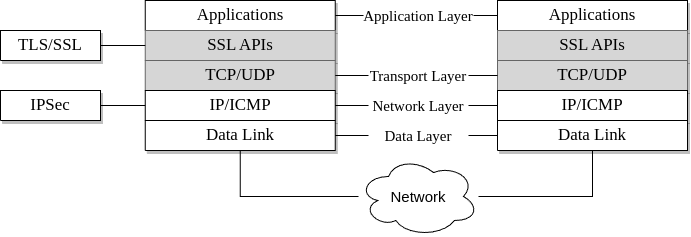
\includegraphics[width= 0.9\textwidth]{figure_3.1}\\
\caption{IPsec's position in the network stack}
\label{fig:figure3.1}
\end{figure}

Operating at the Network layer enables IPsec to provide its services independently of which protocols are utilized at higher layers, while ensuring protection across all layers above it and, optionally including the IP layer.

IPsec defines two protocols: the Authentication Header (AH) \cite{rfc4302} and the Encapsulating Security Protocol (ESP) \cite{rfc4303}. AH offers data integrity, data origin authentication, and optional anti-replay protection, whereas ESP augments AH's functionalities by including data confidentiality \cite{rfc3602}. Utilized cryptographic algorithms include HMAC-SHA1 (\cite{rfc2104}, \cite{rfc4634}, \cite{rfc2404}) and HMAC-MD5 for integrity and authentication, along with AES \cite{fips197} and 3DES for confidentiality. Nevertheless, the framework accommodates the utilization of alternative cryptographic algorithms as needed.

In IPsec, two communication modes are defined: Transport mode and Tunnel mode. Transport mode secures end-to-end communication (Host-to-Host), whereas Tunnel mode extends protection to Network-to-Network and Network-to-Host scenarios. Figures \ref{fig:figure3.2}, \ref{fig:figure3.3}, and \ref{fig:figure3.4} visually depict these communication modes, with the green line denoting the secured segment of the route.

% fig 3.2
\begin{figure}[h!]
\centering
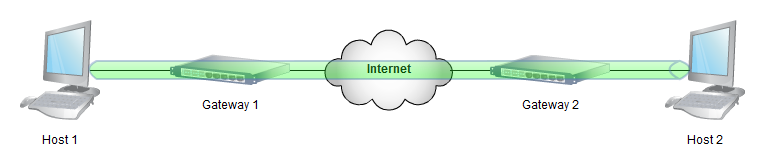
\includegraphics[width= 0.9\textwidth]{figure_3.2}\\
\caption{Host-to-Host in Transport Mode}
\label{fig:figure3.2}
\end{figure}

% fig 3.3
\begin{figure}[h!]
\centering
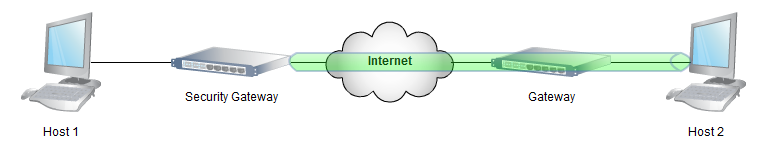
\includegraphics[width= 0.9\textwidth]{figure_3.3}\\
\caption{Network-to-Host in Tunnel Mode}
\label{fig:figure3.3}
\end{figure}


% fig 3.4
\begin{figure}[h!]
\centering
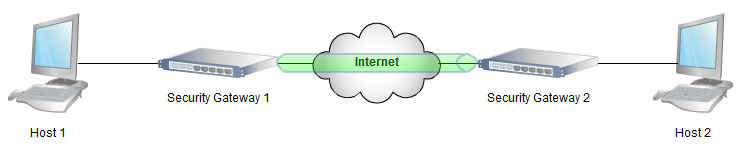
\includegraphics[width= 0.9\textwidth]{figure_3.4}\\
\caption{ Network-to-Network in Tunnel Mode}
\label{fig:figure3.4}
\end{figure}

% Before initiating a secure communication several parameters should be defined and agreed upon. These include the cryptographic algorithms to be used, the keys, the protocol to be applied (AH or ESP), etc. A collection of choices for these security parameters constitutes a Security Association (SA). For each new secure session, an SA should be created at both ends of the communication.

Before initiating secure communication, various parameters must be established and mutually agreed upon, including cryptographic algorithms, keys, and the chosen protocol (AH or ESP). A choice of these security parameters constitutes a Security Association (SA), For each new secure session, an SA should be created at both ends of the communication.

The establishment of SAs within IPsec can be manual or automated. Manual configuration necessitates users to specify parameters at both ends, potentially involving intermediate Security Gateways. Manual configuration has many drawbacks such as maintenance overheads and susceptibility to human errors, hence automated methods are generally favored. The Internet Key Exchange Protocol (IKE) orchestrates automated parameter negotiation, secure key exchange, and maintenance, drawing upon the Oakley and ISAKMP protocols.

Security associations contain the parameters for secure communication. However, they do not determine whether the two ends are legitimate to communicate via IPsec. This determination, as well as whether IPsec should be used in the communication, is defined through the Security Policy (SP) mechanism. Security policies are a management mechanism for IPsec users. Thus, system users define, at a higher level, the nature of communication with other systems, without being concerned with low-level details (algorithms, keys, etc.). The actions defined in IPsec policies are three: Protecting traffic (Apply IPsec, Protect), Bypassing IPsec, or Discarding traffic. Security policies have a set of selectors to filter traffic and determine which policy it belongs to.

While security associations define parameters for secure communication, they do not ascertain when IPsec needs to be used and between which entities. These parameters are controlled through the Security Policy (SP) mechanism. SPs serve as a management framework for IPsec users, allowing higher-level specification of the nature of communication with other systems without delving into low-level details such as algorithms and keys. SPs use 'selectors' to identify what policy to apply to which communication. SPs also define what actions need to be taken for a given communication. The options for SP actions are:
\begin{outline}
    \1 Protect (apply IPsec)
    \1 Bypass (send/process the packet without applying IPsec)
    \1 Discard (do not send/process the packet)
\end{outline}

When implementing IPsec, one has to consider how to integrate it with the rest of the protocol stack. Three options exist:
\begin{outline}
\1 Native:\\
IPsec is implemented within the protocol stack. Access to the stack code is required for integration.
\1 Bump-in-the-stack (BITS):\\
IPsec is implemented "below" a deployed version of the IP layer, between the network layer and the network interface. Access to the source code is not required for this choice. This approach is preferred when integrating IPsec in commercial closed-source products.
\1 Bump-in-the-Wire (BITW):\\
IPsec is implemented in an external device rather than within the systems that utilize it. This method is common in military and some commercial applications. The embedded device acts as an "assistant" to the host system and often has its own IP address.
\end{outline}

\subsection{Outbound Packet Processing}
IPsec defines the flow of outbound packet processing as follows:
\begin{outline}

\1 Initially, information in the header of the outgoing packet is used to identify a policy that can be applied to this traffic. If no matching policy is found, the packet is discarded (Discard action).

\1 If a policy is found, it is applied. If the action is to Bypass, no further action is required by IPsec, and the packet continues its usual path through the stack. If the action is Discard, the packet is dropped. If the action is Protect, the SA pointed by the policy is queried, and the specific security parameters in the SA are used. If no SA is found and if automated SA creation is supported then the key manager (e.g. IKE) gets invoked. If the key manager fails or there is no support for automated SA creation, the action defaults to Discard.

\1 Finally, if the packet has not been discarded, it is sent.
\end{outline}

The flowchart for the above process is presented in Figure \ref{fig:figure3.5}.

% fig 3.5
\begin{figure}
\centering
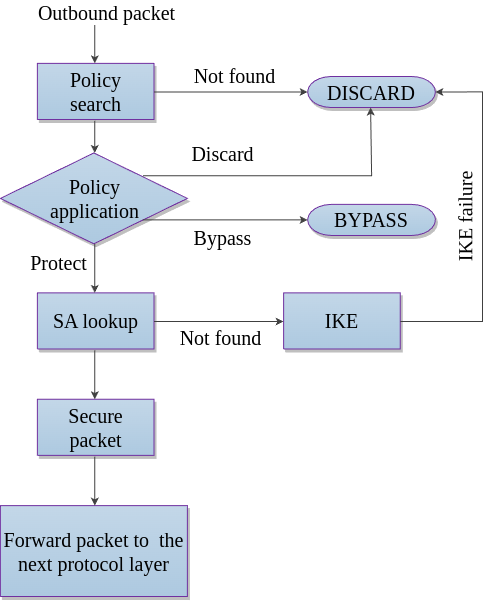
\includegraphics[width= 0.6\textwidth]{figure_3.5}\\
\caption{ Outbound packet processing flowchart}
\label{fig:figure3.5}
\end{figure}

\subsection{Inbound Packet Processing}

IPsec defines the flow of outbound packet processing as follows:
\begin{outline}

\1 Initially, information in the header of the outgoing packet is used to identify a policy that can be applied to this traffic. If no matching policy is found, the packet is discarded (Discard action).

\1 In the case where the policy action is Protect, the corresponding SA is searched using a Security Parameter Index (SPI) present in the incoming packet, and the security parameters in the SA are used. If no SA is found, the packet is discarded.

\1 After applying the SA, the processed packet is checked against its corresponding policy to verify its correct protection.
\end{outline}

The above process is presented in flowchart form in Figure \ref{fig:figure3.6}.

% fig 3.6
\begin{figure}
\centering
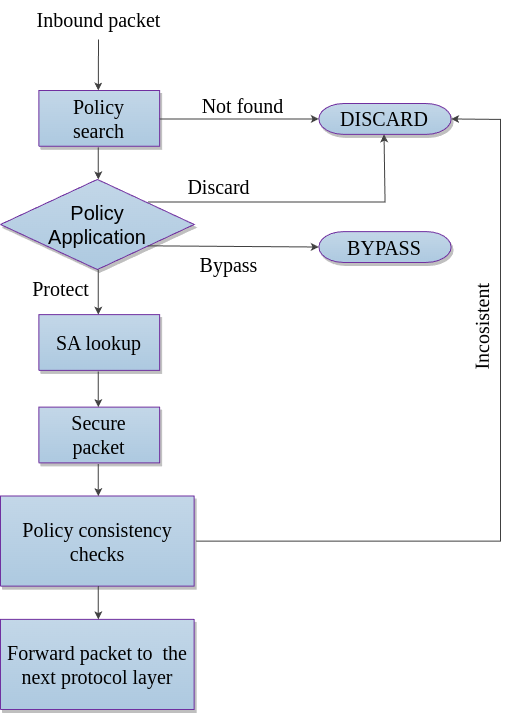
\includegraphics[width= 0.6\textwidth]{figure_3.6}\\
\caption{ Inbound packet processing flowchart}
\label{fig:figure3.6}
\end{figure}

\subsection{Transport and Tunnel Modes}
As previously stated, IPsec protocols can operate in either Transport mode or Tunnel mode. The difference in these two modes lies in which parts of the IP packet are considered the designated "payload" of the IPsec packet. In Transport mode,  only the data of the higher layer is considered as payload, while in Tunnel mode, the payload is extended to include the IP header. Figures \ref{fig:figure3.7} and \ref{fig:figure3.8} illustrate the packet format for Transport and Tunnel mode respectively, for both AH and ESP.

% fig 3.7
\begin{figure}[H]
\centering
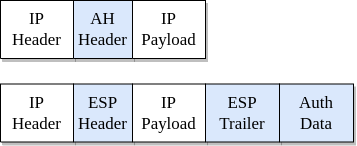
\includegraphics[width= 0.5\textwidth]{figure_3.7}\\
\caption{ AH (up) and ESP (down) packet formats in Transport Mode}
\label{fig:figure3.7}
\end{figure}

% fig 3.8
\begin{figure}[H]
\centering
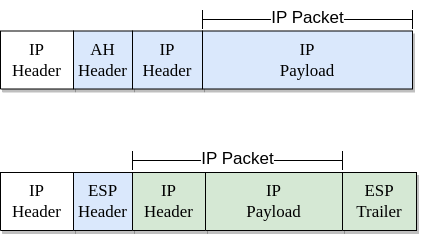
\includegraphics[width= 0.5\textwidth]{figure_3.8}\\
\caption{ AH (up) and ESP (down) packet formats in Tunnel Mode}
\label{fig:figure3.8}
\end{figure}


In transport mode, only the hosts execute IPsec. Initially, the appropriate protection is applied to the packet by the sender, and then the corresponding header is added to the data of the higher protocol. This is followed by the addition of the IP header, and finally, the packet is sent to the destination address. When it reaches the recipient, the packet is processed by IPsec, and the resulting payload is handed to the appropriate higher-layer protocol.

In tunnel mode, one or two Security Gateways (SGs) are involved. In the scenario of network-to-network tunnel mode, two SGs are used. The process starts with the packet being sent by the sender as normal. When the packet reaches the local SG, IPsec protection is applied to the entire IP packet. Then the security protocol header is added at the position right after the original IP header. Subsequently, a new IP header is added, containing the addresses of both the local and remote SGs, and finally packet is transmitted. When the packet reaches the remote SG, it is processed by IPsec, resulting in the original IP packet. Then, the IP packet is forwarded unmodified to the local network to reach its final recipient.

In the network-to-host scenario, where only a single SG is involved, two things change compared to the network-to-network scenario. Firstly, during transmission at the end of the communication where there is no SG, the host assumes SG's processing responsibilities. In other words, the host is effectively acting as its own SG. Secondly, during packet transmission from the SG-equipped end, the SG only routes the packet without applying tunnel mode processing. Thus, in network-to-host scenarios, tunnel mode operates from the host to the SG, transitioning to transport mode from the SG-equipped end to the host.


\section{Security Associations (SA)}
As previously mentioned, a Security Association (SA) is a data structure containing information regarding the parameters governing a security session. SAs encapsulate parameters for each unidirectional session, leading to the utilization of two SAs per node in bidirectional scenarios — one for inbound and one for outbound traffic. These SAs are stored in a database known as the Security Association Database (SADB). Each SA is uniquely identified by a Security Parameter Index (SPI) which is used during search and retrieval of SAs. Both AH and ESP packets have a dedicated field within their headers designated for storing the SPI value corresponding to the applicable SA. SAs can be defined either manually by the system user or automatically through a negotiation protocol. Moreover, they have a lifetime limit, meaning they are invalidated after a certain period, and a new negotiation must start. An SA entry includes:
\begin{outline}
\1 The security protocol used (AH or ESP)
\1 The mode used (Transport or Tunnel)
\1 A Sequence Number for Anti-Replay
\1 Information about the authentication algorithm used in AH, such as the algorithm type, the key id, etc.
\1 Information about the encryption algorithm used in ESP, such as the algorithm's mode, the key id, the initialization vector, etc.
\1 Information about the data integrity algorithm used in ESP
\end{outline}

\section{Security Policy Database (SPD)}
The defined Security Policies are stored in the Security Policy Database (SPD). SPD facilitates the search for the appropriate policy for a specific packet. The order in which policies are stored in the SPD also defines their priority of application. Each security policy is a data structure that holds information used for matching the policy to a specific type of traffic. The specific types of this information are called selectors and they include:
\begin{outline}
\1 lists of local IP addresses
\1 lists of remote IP addresses
\1 higher-layer protocol
\1 local port
\1 remote port
\end{outline}

An SP entry includes:

\begin{outline}
\1 The type of policy to be applied. The three possible values are Protect, Bypass, and Discard. In the case of Protect, additional information is included in the SP:
\2 the IPsec mode
\2 for Tunnel Mode, the local and remote IP addresses of the tunnel
\2 the security protocol to be applied
\2 a prioritized list of algorithms that are allowed to be used. This information is useful in determining which algorithm will be used during an SA negotiation
\2 the SPI of the SA that this policy can use
\end{outline}

\section{The Authentication Header (AH) Protocol}
The AH protocol provides authentication, data integrity, and optional anti-replay protection for IP packets. Protection is provided for most of the IP packet and higher-layer protocol data,  however, since some fields in the IP header can change during transit and thus their final values cannot be predicted, they are committed from AH protection.

AH defines a header format that provides information regarding the packet's protection. The format of the header is shown in Figure \ref{fig:figure3.9}. The fields' purposes are:

\begin{outline}
\1 Next Header: \\The 8-bit standardized number (IANA) of the protocol that AH encapsulates. In tunnel mode, it can take only take the values 4 for IPv4 or 41  for IPv6.
\1 Payload Length: \\An 8-bit field denoting the size of the entire AH packet, expressed as a multiple of 32 bits and reduced by 2.
\1 Reserved: \\Reserved for future use. Mandated to be set to 0 by the sender, with no recipient verification requirement.
\1 Security Parameter Index (SPI):\\ A 32-bit value pointing to the applicable SA.
\1 Sequence Number: \\An unsigned 32-bit integer denoting the packet's sequence number within the SA session. It is used by the anti-Replay mechanism. The field is mandatory, even when anti-replay is decativated.
\1 Authentication Data (or Integrity Check Value – ICV):\\ A variable-sized field containing the outcome of the integrity/authentication algorithm. This field must be an integer multiple of 32 bits. Padding is included for proper alignment of the packet on a 32-bit boundary.
\end{outline}

% fig 3.9
\begin{figure}[H]
\centering
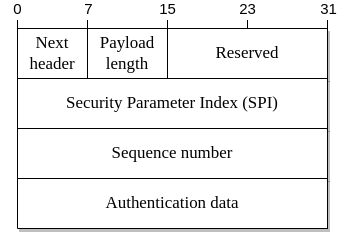
\includegraphics[width= 0.5\textwidth]{figure_3.9}\\
\caption{ Structure of the AH protocol header }
\label{fig:figure3.9}
\end{figure}

\subsection{Outbound Packet Processing}
The outbound packet processing for AH is as follows:
\begin{outline}[enumerate]
\1 Finding SA: \\The AH protocol is applied when the SA corresponding to this traffic designates it as the protocol.

\1 Sequence Number calculation:\\ The sender starts the Sequence Number counter at 0 and increments it by 1 for each subsequent outgoing packet. Its value is stored in the SA. In the case of automatic SA creation and if the counter has returned to 0 after traversing all values, the SA expires and a new one must be created. If SA management is manual, then the counter restarts from 0.

\1 ICV calculation: \\Calculation of the ICV involves the payload, the AH header, and a portion of the outer IP header. The value of the Authentication Data field is assumed to be all zeros for this calculation. From the IP header, only the fields that remain constant in the packet's path (immutable) are selected. The rest (mutable), their values are assumed as 0. The mutable fields of the IPv4 header are TOS, Flags, Fragment Offset, TTL, and Header Checksum. For IPv6, they are TOS, Flow Label, and Hop Limit. The calculated ICV value is placed in the Authentication Data field.

\1 Padding: \\Finally, if necessary, padding is applied to ICV so that the entire packet is a multiple of 32 bits in IPv4 and a multiple of 64 bits in IPv6. Additional padding may be required to make the packet size a multiple of the block size of the algorithm used for authentication/integrity.
\end{outline}

\subsection{Inbound Packet Processing}
The inbound packet processing for AH is as follows:
\begin{outline}[enumerate]
\1 Finding SA:\\ Firstly, SPI is used to locate an applicable SA. If no SA is found, the packet is discarded.

\1 Anti-replay:\\ If the anti-replay protection is enabled, the Sequence Number is checked. If found correct the processing continues; otherwise, the packet is discarded.

\1 ICV verification:\\ The receiver calculates the ICV in the same way as the sender. It then checks if the calculated value matches the value contained in the packet. If they do not match, then some alteration has occurred during the packet's transmission, and the packet is discarded.
\end{outline}

\section{The Encapsulation Security Payload (ESP) Protocol}
The ESP protocol provides authentication, data integrity, confidentiality, and optionally anti-replay protection. The set of services it provides is determined by the corresponding SA. Authentication and integrity are always provided together, which makes three combinations of services possible:
\begin{outline}
\1 Confidentiality only
\1 Authentication-integrity only
\1 Confidentiality and authentication-integrity
\end{outline}

ESP uses both a header and a trailer for the packet. The format of an ESP packet is shown in Figure \ref{fig:figure3.10}. The fields' purposes are:
\begin{outline}
\1 SPI: \\As with AH, this is the index for the corresponding SA.
\1 Sequence Number:\\ As with AH, this is the incrementing number for the anti-replay protection.
\1 IV (Initialization Vector):\\ This is an optional field. It is used when an IV is required by the encryption algorithm.
\1 Padding: \\ This field has two purposes. If a block encryption algorithm is used, it aligns the packet to the block size. Otherwise, it aligns the packet to a multiple of 32 bits. The contents of the padding bytes are determined either by the encryption algorithm or the default padding is used. This default padding is the monotonically increasing integer sequence starting from 1.
\1 Pad Length: \\ This field holds the length of the padding field in, expressed in bytes.
\1 Next Header: \\ The IANA number of the higher-layer protocol.
\1 Authentication Data: \\ A variable size field containing the result of the authentication/integrity algorithm. The size of this field is determined by the specific algorithm.
\end{outline}

% fig 3.10
\begin{figure}
\centering
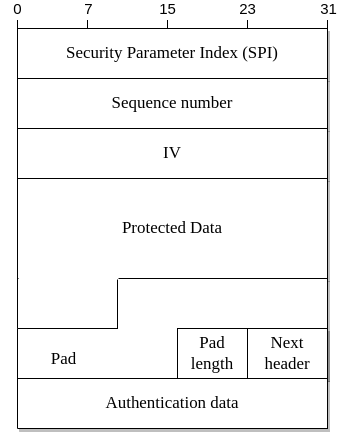
\includegraphics[width= 0.5\textwidth]{figure_3.10}\\
\caption{ Structure of the ESP protocol header }
\label{fig:figure3.10}
\end{figure}

\subsection{Outbound Packet Processing}

During outbound packet processing, once the SA corresponding to the outgoing packet is found and if the SA specifies the use of the ESP protocol, the following actions are taken:

\begin{outline}[enumerate]
\1 Padding is initially applied to the payload, so that the packet size becomes a multiple of 32 or 64 bits (for IPv4 and IPv6 respectively), or so that it becomes a multiple of the block size of the encryption algorithm. Additionally, the Payload Length and Next Header fields are inserted.

\1 Next, if confidentiality is required, the encryption algorithm is executed on the payload. The corresponding key, and, if required, IV, are provided by the SA.

\1 If an IV is required, it is placed at the start of the payload, following the ESP header.

\1 The Sequence Number is then calculated and the ESP header is inserted.

\1 Finally, if an authentication/integrity is required, the ICV is computed over the header and payload of the packet, and the result is placed in the trailer's Authentication Data field. The key and any other data needed by the algorithm are provided by the SA.
\end{outline}

\subsection{Inbound Packet Processing}
To begin processing an incoming packet with ESP, the corresponding SA must first be found and must specify that ESP processing needs to take place. If no SA is found, the packet is discarded. Otherwise, the following steps are taken:
\begin{outline}[enumerate]
\1 Initially, if anti-replay protection is used, the Sequence Number value is checked. If found correct, the packet processing continues. Otherwise, the packet is rejected.

\1 If authentication/integrity is used, the ICV of the packet is computed and compared with the ICV value in the packet. The key is provided by the SA. If the ICV values match, the packet passes the authentication/integrity check; otherwise, it is rejected.

\1 Next, if confidentiality is used, the decryption algorithm is executed using the key provided by the SA and, if available, the IV contained in the packet.

\1 Finally, the padding is removed and the result is the plaintext payload.
\end{outline}

\section{Key Management}
In IPsec, key management is performed using the Internet Key Exchange (IKE) protocol. IKE is a complex protocol based on the Oakley and ISAKMP protocols. Its purpose is the automated creation and management of Security Associations (SAs). Its main responsibilities include:

\begin{outline}
\1 Creating new SAs: This is achieved through a series of negotiations between the two communication ends regarding communication parameters such as authentication and encryption algorithms, keys, etc.
\1 Monitoring SA expiration and renegotiating them.
\end{outline}

IKE is executed in two phases. First, ISAKMP is used to generate an ISAKMP Security Association which establishes a secure communication channel. Then, this secure channel is used to negotiate IPsec SAs, in pairs. The first phase has various execution modes, namely Main Mode, Aggressive Mode, and Base Mode. Each mode is defined as a series of messages consisting of various headers and payloads. The second phase has only one mode, Quick Mode. Additionally, there are other message exchanges for various IKE functions that are not part of these two phases, such as New Groups Mode, Unacknowledged Notification exchanges, and Acknowledged Notification exchanges.

Before IKE executes, the identities of the two ends must be authenticated. IKE uses three methods for authentication: a pre-shared secret key, digital signatures, or public key encryption.
